\chapter{Конструкторская часть}
\label{cha:design}

\section{Разработка алгоритмов}

В данном разделе будут рассмотрены схемы.

На рис. \ref{ref:d0} показана схема алгоритма полного перебора.

\begin{figure}[ht!]
	\centering{
		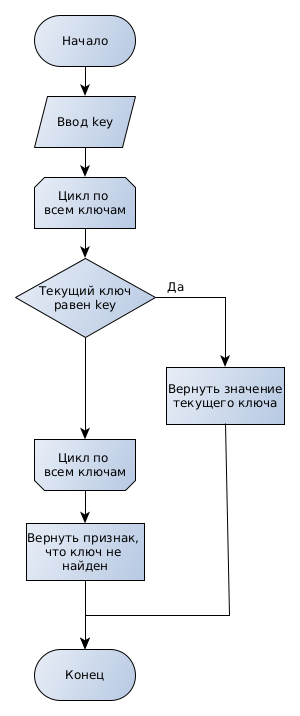
\includegraphics[width=1\textwidth]{d1.png}
		\caption{Схема алгоритма полного перебора}
		\label{ref:d0}}
\end{figure}

На рис. \ref{ref:d1} показана схема муравьиного алгоритма.

\begin{figure}[ht!]
	\centering{
		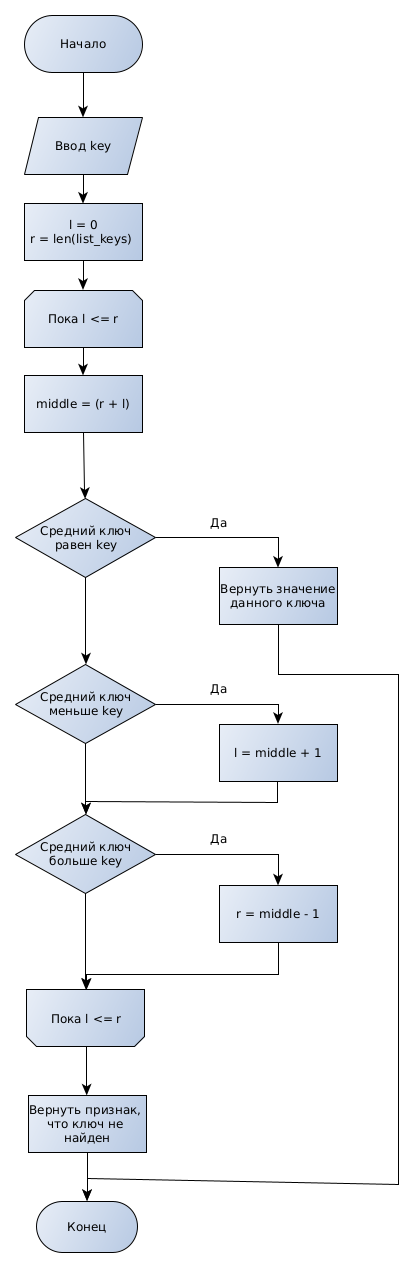
\includegraphics[width=0.9\textwidth]{d2.png}
		\caption{Схема муравьиного алгоритма}
		\label{ref:d1}}
\end{figure}

\section{Вывод}

В данном разделе были рассмотрены схемы алгоритма полного перебора \ref{ref:d0}
и схема муравьиного алгоритма \ref{ref:d1}.






